% =====================================================================
%  Strona tytułowa — TREŚĆ (per-dokument). Tytuł, PODPIS AUTOREM, wykres.
% =====================================================================
\begin{titlepage}
\centering
\vspace*{1.2cm}

\slayertitle
  {Tytuł empirycznego raportu}% tytuł
  {Autor / kolektyw Slayer}% PODPIS autorem
  {\today}% data

\vspace{1.4cm}

% --- WYKRES NA PIERWSZEJ STRONIE + PODPIS (rdzeń: empiria od razu widoczna) ---
\begin{figure}[h]
  \centering
  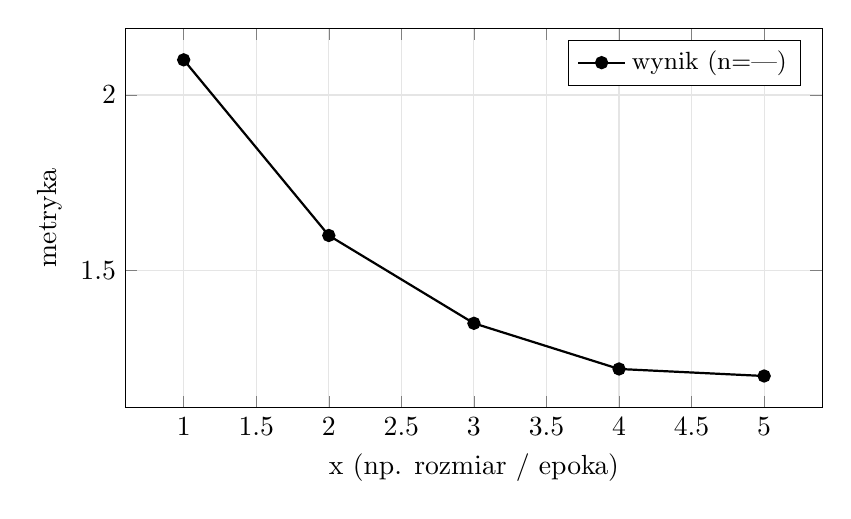
\begin{tikzpicture}
    \begin{axis}[
        width=0.86\linewidth, height=6.4cm,
        xlabel={x (np. rozmiar / epoka)}, ylabel={metryka},
        grid=both, grid style={gray!20},
        legend pos=north east, legend style={font=\small},
    ]
      % DANE PRZYKŁADOWE — podmień na realne.
      \addplot[thick,mark=*] coordinates {(1,2.1)(2,1.6)(3,1.35)(4,1.22)(5,1.20)};
      \addlegendentry{wynik (n=---)}
    \end{axis}
  \end{tikzpicture}
  \caption{\textbf{Wynik empiryczny --- podpis pod wykresem.} Co pokazuje, na jakich
  danych, jednostki. Dane \emph{przykładowe} (do podmiany na realne). Tu mieszka
  „pierwsze wrażenie" dokumentu --- niech wykres mówi tezę.}
  \label{fig:hero}
\end{figure}

\vfill
{\small Slayer · dokument kompilowany w CI do PDF · matematyka w \texttt{\$...\$}}
\end{titlepage}
